% =====================================================================
%  MARS: Multi-Agent Framework for Reliable Radiological Segmentation
%        and Report Generation
%  Overleaf-ready LaTeX source. Compile with pdfLaTeX (or XeLaTeX).
% =====================================================================
\documentclass[11pt,a4paper]{article}

% ---------------------------------------------------------------------
% Packages
% ---------------------------------------------------------------------
\usepackage[margin=1in]{geometry}
\usepackage[utf8]{inputenc}
\usepackage[T1]{fontenc}
\usepackage{lmodern}
\usepackage{amsmath,amssymb,amsthm}
\usepackage{graphicx}
\usepackage{booktabs}
\usepackage{array}
\usepackage{multirow}
\usepackage{longtable}
\usepackage{xcolor}
\usepackage{hyperref}
\usepackage{enumitem}
\usepackage{caption}
\usepackage{subcaption}
\usepackage{tcolorbox}
\usepackage{listings}
\usepackage{tikz}
\usepackage{pgfplots}
\pgfplotsset{compat=1.17}
\usetikzlibrary{arrows.meta,positioning,shapes.geometric,fit,backgrounds,calc}
\usepackage{titlesec}
\usepackage{fancyhdr}
\usepackage{abstract}
\usepackage{doi}

\tcbuselibrary{skins,breakable}

% ---------------------------------------------------------------------
% Colors
% ---------------------------------------------------------------------
\definecolor{mrsblue}{RGB}{25,71,138}
\definecolor{mrsteal}{RGB}{20,130,130}
\definecolor{mrsamber}{RGB}{201,132,17}
\definecolor{mrsgreen}{RGB}{46,125,50}
\definecolor{mrsred}{RGB}{176,42,42}
\definecolor{mrsgrey}{RGB}{240,242,245}
\definecolor{mrsviolet}{RGB}{106,66,166}

\hypersetup{
  colorlinks=true,
  linkcolor=mrsblue,
  citecolor=mrsteal,
  urlcolor=mrsblue,
  pdftitle={MARS: Multi-Agent Framework for Reliable Radiological Segmentation and Report Generation},
  pdfauthor={Trupti Agrawal, Trupthi Mantri, Navya Sree Balu, Ankam Hitha}
}

\lstset{
  basicstyle=\ttfamily\footnotesize,
  breaklines=true,
  frame=single,
  columns=fullflexible,
  numbers=left,
  numberstyle=\tiny\color{gray},
  keywordstyle=\color{mrsblue}\bfseries,
  commentstyle=\color{gray}\itshape,
  stringstyle=\color{mrsgreen},
  backgroundcolor=\color{mrsgrey},
}

\newtcolorbox{formulabox}[1][]{
  colback=mrsgrey, colframe=mrsblue!70!black, boxrule=0.6pt,
  arc=2pt, left=6pt, right=6pt, top=4pt, bottom=4pt,
  title={#1}, fonttitle=\bfseries\small, coltitle=white,
  colbacktitle=mrsblue, breakable
}

\newtcolorbox{keytakeaway}[1][Key Takeaway]{
  colback=mrsamber!10, colframe=mrsamber!80!black, boxrule=0.6pt,
  arc=2pt, left=6pt, right=6pt, top=4pt, bottom=4pt,
  title={#1}, fonttitle=\bfseries\small, coltitle=white,
  colbacktitle=mrsamber!90!black, breakable
}

\newcounter{algcount}
\newtcolorbox[use counter=algcount]{algobox}[2][]{
  colback=white, colframe=mrsblue!70!black, boxrule=0.6pt,
  arc=2pt, left=8pt, right=8pt, top=5pt, bottom=5pt,
  title={Algorithm~\thetcbcounter: #2}, fonttitle=\bfseries\small,
  coltitle=white, colbacktitle=mrsblue, breakable, #1
}
\newenvironment{algosteps}{\begin{enumerate}[label=\arabic*:, leftmargin=2.1em, itemsep=1pt, topsep=2pt]}{\end{enumerate}}
\newcommand{\algoreturn}[1]{\textbf{return} #1}
\newcommand{\algoif}[1]{\textbf{if} #1 \textbf{then}}
\newcommand{\algoelse}{\textbf{else}}
\newcommand{\algocomment}[1]{\hfill\textcolor{gray}{\footnotesize $\triangleright$ #1}}

\titleformat{\section}{\large\bfseries\color{mrsblue}}{\thesection}{0.6em}{}
\titleformat{\subsection}{\normalsize\bfseries\color{mrsblue!80!black}}{\thesubsection}{0.6em}{}

\pagestyle{fancy}
\fancyhf{}
\fancyhead[L]{\small\textit{MARS: Multi-Agent Reliable Segmentation \& Reporting}}
\fancyhead[R]{\small\thepage}
\renewcommand{\headrulewidth}{0.3pt}

\title{\textbf{\Large MARS: A Multi-Agent Framework for Reliable Radiological\\
Segmentation, Clinical Validation, and Uncertainty-Aware\\
Report Generation in CT Imaging}}

\author{
Trupti Agrawal$^{1}$ \quad Trupthi Mantri$^{1}$ \quad Navya Sree Balu$^{1}$ \quad Ankam Hitha$^{1}$\\[4pt]
\small $^{1}$Department of Information Technology, BVRIT Hyderabad College of Engineering for Women\\
\small Guide: Dr.\ K.\ Srikar Goud, Assistant Professor, Dept.\ of IT\\
\small\texttt{\{23wh1a1277, 23wh1a1271, 23wh1a1286, 23wh1a1289\}@bvrithyderabad.edu.in}
}
\date{September 2026}

% =====================================================================
\begin{document}
\maketitle

\begin{abstract}
\noindent
Deep-learning segmentation models routinely match expert-level accuracy on lesion delineation from CT scans, yet adoption in clinical workflow remains limited. The bottleneck is not raw accuracy but \emph{trust}: a segmentation mask is delivered with no honest signal of how much it should be believed, forcing a radiologist to either verify every case (eliminating the time saved) or verify none (an unsafe default). We present \textbf{MARS} (Multi-Agent framework for Reliable segmentation and report generation), a four-agent pipeline that decomposes CT lesion analysis into \emph{Segmentation}, \emph{Clinical Validation}, \emph{Uncertainty Aggregation}, and \emph{Reporting/Routing} agents, each producing an explicit, inspectable output. The Segmentation agent is architected around \textbf{Slide-SAM}, a sliding-window adaptation of the Segment Anything Model (SAM) for 3D medical volumes, while the Validation agent cross-checks every predicted mask against structured clinical metadata (expected anatomical site, expected lesion size) to catch confidently-wrong predictions that segmentation confidence alone cannot detect. A calibrated scalar uncertainty $U$ is then computed from the two upstream signals and compared against a configurable safety threshold $\tau$, routing each case to an automated report or to radiologist escalation with an explicit reason. We describe the system architecture, the configuration and data schema, algorithmic detail for every agent, and a reproducible synthetic-volume evaluation harness used to validate pipeline mechanics ahead of full clinical-data training. We further present a truthful, limitation-aware comparison between vanilla SAM, Slide-SAM, and the proposed multi-agent wrapper, and outline the calibration-focused evaluation protocol (Dice/IoU/Hausdorff, Expected Calibration Error, risk--coverage analysis) planned for the trained system. MARS treats ``knowing when it does not know'' as a first-class design requirement rather than a post-hoc addition.
\end{abstract}

\noindent\textbf{Keywords:} medical image segmentation, multi-agent systems, Segment Anything Model (SAM), Slide-SAM, uncertainty quantification, clinical decision support, CT imaging, selective prediction.

\tableofcontents
\vspace{1em}
\hrule

% =====================================================================
\section{Introduction}
\label{sec:intro}

\subsection{Problem Statement}
Convolutional and transformer-based segmentation networks can now delineate lesions in CT volumes with Dice scores rivaling inter-radiologist agreement \cite{sam,sam2}. Despite this, such models rarely enter routine hospital workflow. The obstacle is not model accuracy but the absence of a trustworthy \emph{reliability signal} attached to each prediction. A segmentation network outputs a mask $M$; it does not, by itself, output an honest estimate of how much that mask should be trusted. This leaves a radiologist with two unattractive options:

\begin{itemize}[leftmargin=1.4em]
    \item \textbf{Verify every prediction manually} --- the AI system saves no clinical time, removing the incentive to deploy it at all.
    \item \textbf{Verify none of them} --- clinically unsafe, since a single silent failure on one scan can produce a missed or mis-staged lesion.
\end{itemize}

A second, related gap is that a segmentation mask is not a diagnosis. Segmentation performed in isolation ignores the patient's clinical context (expected lesion site, prior history, expected size) and produces nothing a clinician can directly place in a case file. The reporting step --- where the clinical value of the pipeline actually lands --- is typically missing from segmentation-only research systems.

\subsection{Formal Problem Formulation}
Given a 3D CT volume $X \in \mathbb{R}^{D\times H\times W}$ and structured clinical metadata $C$, MARS defines the following functional decomposition:

\begin{formulabox}[Problem Formulation]
\begin{align}
M &= f_{\text{seg}}(X) &&\text{volumetric segmentation mask} \label{eq:seg}\\
V &= f_{\text{val}}(M, C) &&\text{clinical consistency score} \label{eq:val}\\
U &= f_{\text{unc}}(M, V, C) &&\text{scalar prediction uncertainty} \label{eq:unc}\\
D &=
\begin{cases}
\text{Automated report}, & U < \tau \\
\text{Expert (radiologist) review}, & U \geq \tau
\end{cases} &&\text{routing decision} \label{eq:route}
\end{align}
\end{formulabox}

\noindent where $\tau \in [0,1]$ is a configurable safety threshold. The objective is to generate precise volumetric segmentation masks \emph{while concurrently} quantifying prediction uncertainty, then to compare that uncertainty against $\tau$ to dynamically route each case between automated processing and expert review.

\subsection{Contributions}
This work makes the following contributions:

\begin{enumerate}[leftmargin=1.4em]
    \item \textbf{A four-agent architecture} that separates segmentation, clinical validation, uncertainty aggregation, and reporting into independently replaceable, independently evaluable components (Sections~\ref{sec:overview}--\ref{sec:design}), in contrast to prior work that treats SAM-based CT segmentation as a single, monolithic step \cite{caroline,slidesam}.
    \item \textbf{A clinically-grounded validation agent} that flags anatomically or dimensionally implausible masks using structured metadata, catching confidently-wrong predictions that per-voxel segmentation confidence alone cannot detect.
    \item \textbf{A calibrated uncertainty-aggregation formulation} that fuses segmentation confidence and clinical consistency into a single scalar $U$ with per-factor attribution, and an accompanying evaluation protocol (Expected Calibration Error, risk--coverage curves) that treats calibration, not just accuracy, as a first-class metric.
    \item \textbf{An explainable routing and reporting layer} in which every escalation carries a specific, human-readable reason rather than a bare ``low confidence'' flag.
    \item \textbf{A reproducible synthetic-volume harness} (deterministic seeding, versioned schema) used to validate pipeline mechanics end-to-end prior to training on annotated clinical CT data, together with a truthful SAM vs.\ Slide-SAM comparison that motivates the choice of Slide-SAM as the architectural base for Agent~1.
\end{enumerate}

\subsection{Objectives}
\begin{enumerate}[leftmargin=1.4em]
    \item Perform accurate pixel-level lesion segmentation on CT scans, with per-prediction confidence scores.
    \item Validate every generated mask against the patient's clinical history for anatomical and dimensional consistency.
    \item Estimate the system's own uncertainty so reliable and unreliable cases can be statistically separated.
    \item Route confident cases through automatically and refer uncertain cases to a radiologist, with an explicit reason.
    \item Generate a structured, explainable radiological report for each automatically-cleared case.
\end{enumerate}

\subsection{Scope}
\textbf{In scope:} lesion segmentation on 3D CT volumes; per-voxel and per-case confidence estimation; consistency checking against structured clinical metadata; threshold-based routing; structured report generation with traceable reasoning.
\textbf{Out of scope (v1):} modalities other than CT (MRI, X-ray, ultrasound); real-time intra-operative use; final diagnostic authority (MARS supports a radiologist, it does not replace one); deployment on hospital PACS infrastructure or regulatory clearance.

% =====================================================================
\section{Review of Literature}
\label{sec:lit}

Table~\ref{tab:litreview} summarizes the six works this paper builds on and positions MARS relative to each.

\begin{table}[htbp]
\centering
\caption{Summary of reviewed literature and identified gaps.}
\label{tab:litreview}
\small
\begin{tabular}{p{2.9cm}p{4.6cm}p{4.9cm}}
\toprule
\textbf{Work} & \textbf{Core idea} & \textbf{Limitation MARS addresses} \\
\midrule
Segment Anything (SAM) \cite{sam} & Foundation model for promptable 2D segmentation, trained on 1B+ masks; zero-shot generalization via points/boxes/masks as prompts. & Natively 2D; no notion of volumetric consistency, clinical context, or calibrated uncertainty. \\
SAM~2 \cite{sam2} & Extends SAM with a streaming memory mechanism for video/temporal segmentation, improving object permanence across frames. & Designed for RGB video, not CT intensity statistics; still no clinical validation or routing layer. \\
SAM~3 \cite{sam3} & Concept-level, promptable segmentation grounded in open-vocabulary text/exemplar concepts. & Concept grounding is generic, not tuned to anatomical priors; no self-reported reliability estimate. \\
Training-free Prompt Placement by Propagation (Caroline Meg et al.) \cite{caroline} & Automatically propagates SAM prompts across CT slices without retraining, enabling efficient 3D bone-CT segmentation. & Segmentation only --- no clinical validation, uncertainty estimation, or report generation. \\
Slide-SAM \cite{slidesam} & Adapts SAM to 3D medical volumes via a three-slice sliding window and minimal box prompts, using parameter-efficient adaptation to retain pretrained SAM knowledge. & Requires task-specific fine-tuning; sensitive to large inter-slice spacing and prompt-propagation drift; still a single-stage segmenter with no downstream clinical reasoning. \\
Multi-Agent LLM + Medical Flowcharts for Self-Triage \cite{triage} & Combines LLMs with clinical flowcharts in a multi-agent pipeline for patient self-triage decisions. & Text/symptom-based triage, not imaging; establishes the multi-agent-for-clinical-decisions pattern that MARS adapts to volumetric segmentation. \\
\bottomrule
\end{tabular}
\end{table}

\subsection{Synthesis}
Two independent threads motivate MARS. First, the SAM family \cite{sam,sam2,sam3} and its CT-domain adaptations \cite{caroline,slidesam} establish that promptable segmentation can reach strong zero-/few-shot accuracy on medical volumes without full retraining, but every one of these systems stops at the mask: none report a calibrated reliability score, and none check the mask against anything the clinician already knows about the patient. Second, multi-agent clinical-decision systems such as \cite{triage} demonstrate that decomposing a diagnostic pipeline into cooperating, single-responsibility agents improves explainability and lets each stage be validated independently — but that pattern has, to our knowledge, not been applied to volumetric segmentation with an explicit uncertainty-routing agent. MARS closes this gap by using \textbf{Slide-SAM as the architectural base of Agent~1} (motivated by its strong 3D CT performance under minimal prompting, discussed further in Section~\ref{sec:comparison}) and wrapping it with three additional agents --- validation, uncertainty aggregation, and reporting/routing --- that together turn a bare mask into a governed clinical decision.

% =====================================================================
\section{System Overview}
\label{sec:overview}

MARS ingests a 3D CT volume $X$ together with optional structured clinical metadata $C$ (expected lesion site, expected size range, prior history) and produces one of two outcomes per case: an automatically generated structured report, or an escalation packet for radiologist review that names the specific reason the system withheld automatic clearance. Table~\ref{tab:reqs} restates the governing functional and non-functional requirements that shaped the design.

\begin{table}[htbp]
\centering
\caption{Selected functional (FR) and non-functional (NFR) requirements.}
\label{tab:reqs}
\small
\begin{tabular}{p{1.4cm}p{10.5cm}}
\toprule
\textbf{ID} & \textbf{Requirement} \\
\midrule
FR-2 & The system shall generate a voxel-level lesion segmentation mask. \\
FR-4 & The system shall validate each mask against clinical metadata and report detected inconsistencies. \\
FR-5 & The system shall compute a single aggregate uncertainty value per case. \\
FR-6 & The system shall route each case to the automated or expert path based on a configurable threshold $\tau$. \\
NFR-1 & \textbf{Calibration} --- uncertainty must correlate measurably with actual error; evaluated explicitly. \\
NFR-3 & \textbf{Safety bias} --- when in doubt, escalate. False escalations are acceptable; silent false negatives are not. \\
NFR-4 & \textbf{Modularity} --- each agent is independently replaceable and independently evaluable. \\
NFR-6 & \textbf{Configurability} --- $\tau$ is adjustable without retraining. \\
\bottomrule
\end{tabular}
\end{table}

\begin{keytakeaway}
The system-level success criterion is not raw segmentation accuracy but the \emph{operating point} it buys: at what escalation rate does the auto-cleared subset reach clinically acceptable accuracy? A system escalating 30\% of cases while being near-perfect on the remaining 70\% is a success; one escalating only 5\% while still erring on the rest is not.
\end{keytakeaway}

% =====================================================================
\section{Architecture}
\label{sec:architecture}

Figure~\ref{fig:architecture} shows the end-to-end MARS pipeline. Each agent has exactly one responsibility and passes an explicit, typed, inspectable output forward, so that when the system is unsure, it is possible to say precisely \emph{where} that uncertainty originated.

\begin{figure}[htbp]
\centering
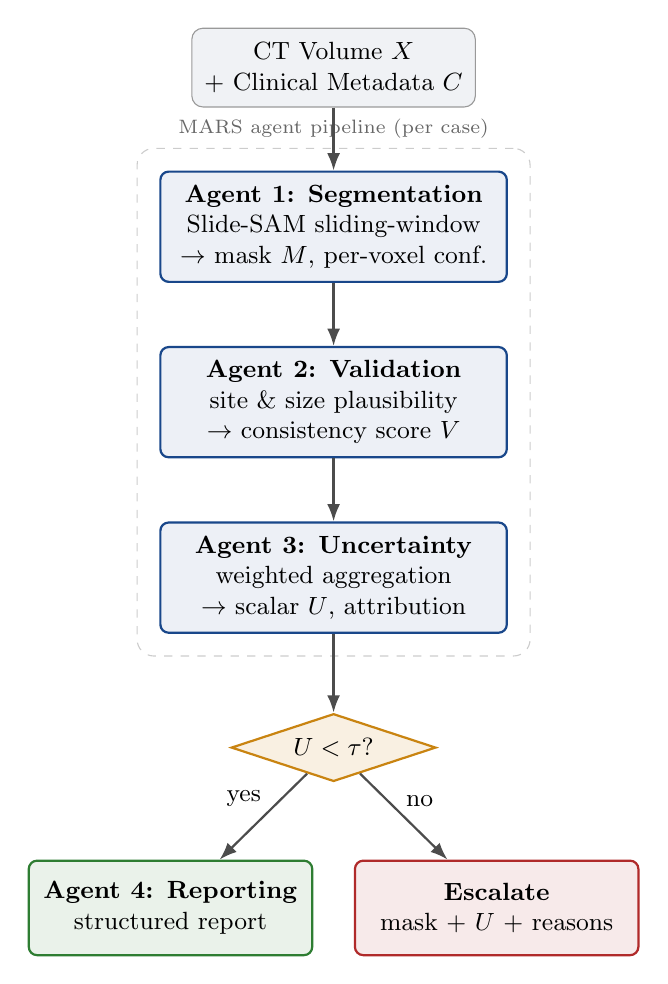
\begin{tikzpicture}[
  node distance=8mm and 14mm,
  every node/.style={font=\small},
  input/.style={rectangle, rounded corners, draw=mrsgrey!0, fill=mrsgrey, minimum width=3.6cm, minimum height=1cm, align=center, draw=black!40},
  agent/.style={rectangle, rounded corners=3pt, draw=mrsblue, thick, fill=mrsblue!8, minimum width=4.4cm, minimum height=1.4cm, align=center},
  decision/.style={diamond, draw=mrsamber, thick, fill=mrsamber!12, aspect=2.4, minimum width=2.6cm, align=center, inner sep=2pt},
  outbox/.style={rectangle, rounded corners=3pt, draw=mrsgreen, thick, fill=mrsgreen!10, minimum width=3.6cm, minimum height=1.2cm, align=center},
  escbox/.style={rectangle, rounded corners=3pt, draw=mrsred, thick, fill=mrsred!10, minimum width=3.6cm, minimum height=1.2cm, align=center},
  arr/.style={-{Latex[length=2.2mm]}, thick, draw=black!70}
]

\node[input] (input) {CT Volume $X$ \\ + Clinical Metadata $C$};
\node[agent, below=of input] (seg) {\textbf{Agent 1: Segmentation}\\ Slide-SAM sliding-window\\ $\rightarrow$ mask $M$, per-voxel conf.};
\node[agent, below=of seg] (val) {\textbf{Agent 2: Validation}\\ site \& size plausibility\\ $\rightarrow$ consistency score $V$};
\node[agent, below=of val] (unc) {\textbf{Agent 3: Uncertainty}\\ weighted aggregation\\ $\rightarrow$ scalar $U$, attribution};
\node[decision, below=10mm of unc] (dec) {$U < \tau$?};
\node[outbox, below left=12mm and -4mm of dec] (auto) {\textbf{Agent 4: Reporting}\\ structured report};
\node[escbox, below right=12mm and -4mm of dec] (esc) {\textbf{Escalate}\\ mask + $U$ + reasons};

\draw[arr] (input) -- (seg);
\draw[arr] (seg) -- (val);
\draw[arr] (val) -- (unc);
\draw[arr] (unc) -- (dec);
\draw[arr] (dec) -- node[above left, xshift=1mm]{yes} (auto);
\draw[arr] (dec) -- node[above right, xshift=-1mm]{no} (esc);

\begin{scope}[on background layer]
\node[fit=(seg)(val)(unc), inner sep=8pt, draw=black!20, dashed, rounded corners=6pt, label={[font=\scriptsize, text=black!60]above:MARS agent pipeline (per case)}] {};
\end{scope}
\end{tikzpicture}
\caption{MARS architecture. Each stage emits a typed Pydantic object consumed by the next; the routing decision at Agent~4 is fully attributable to Agent~3's breakdown.}
\label{fig:architecture}
\end{figure}

\subsection{Component Responsibilities}
\begin{description}[leftmargin=1.6em, style=nextline]
\item[Agent 1 --- Segmentation] Input: 3D CT volume $X$. Output: mask $M$ plus per-voxel and aggregate confidence. Architected around Slide-SAM's sliding three-slice window so pretrained SAM knowledge is retained while gaining volumetric context (Section~\ref{sec:comparison}).
\item[Agent 2 --- Validation] Input: mask $M$, clinical metadata $C$. Output: consistency score $V \in [0,1]$ and an explicit list of conflicts (e.g. anatomically implausible location, size outside expected range). This is the agent that catches a \emph{confidently-wrong} prediction: a model can be certain about a mask in an anatomically implausible location, and segmentation confidence alone will not flag that.
\item[Agent 3 --- Uncertainty] Input: Agent 1's confidence, Agent 2's consistency score. Output: scalar $U$ with per-factor attribution (\texttt{dominant\_factor}). This is the core reliability contribution: $U$ is only meaningful if it is \emph{calibrated}, i.e.\ high $U$ measurably correlates with high error.
\item[Agent 4 --- Reporting / Routing] Input: $M$, $U$, validation findings, threshold $\tau$. Output: either a structured report ($U < \tau$) or an escalation packet naming the specific reason for the doubt ($U \geq \tau$).
\end{description}

% =====================================================================
\section{Methodology: Configuration and Data Schema}
\label{sec:methodology}

MARS is implemented as a Python package (\texttt{mars}) with each agent as a pure function over strongly-typed Pydantic models, so that every intermediate artifact is both machine-validated and directly serializable to a relational or document store. This section shows the schema and configuration surface exactly as implemented in the reference codebase, so results in later sections are reproducible.

\subsection{Case Configuration}
Table~\ref{tab:config} lists the tunable parameters exposed by the pipeline, none of which require retraining a model to change (satisfying NFR-6).

\begin{table}[htbp]
\centering
\caption{Pipeline configuration parameters.}
\label{tab:config}
\small
\begin{tabular}{lp{3.6cm}p{4.6cm}p{2.4cm}}
\toprule
\textbf{Parameter} & \textbf{Meaning} & \textbf{Effect} & \textbf{Default} \\
\midrule
$\tau$ (\texttt{tau}) & routing safety threshold & lower $\tau$ pushes more cases to expert review & $0.5$ \\
\texttt{threshold} & segmentation intensity cut & voxels above this value are candidate lesion & $120.0$ \\
$w_{\text{confidence}}$ & weight of segmentation confidence in $U$ & higher $\Rightarrow$ $U$ dominated by mask quality & $0.5$ \\
$w_{\text{consistency}}$ & weight of clinical consistency in $U$ & higher $\Rightarrow$ $U$ dominated by clinical plausibility & $0.5$ \\
\texttt{SITES} & expected $z$-fraction range per anatomical site & defines the plausibility window used by Agent~2 & anterior $[0,0.5]$, posterior $[0.5,1]$ \\
\bottomrule
\end{tabular}
\end{table}

\subsection{Data / Schema Design}
Every agent boundary is a validated schema, which doubles as the natural relational-database design for a production deployment (Table~\ref{tab:schema}). This directly satisfies NFR-2 (explainability) and NFR-4 (modularity): any agent can be swapped for an alternative implementation as long as it honors the same schema.

\begin{table}[htbp]
\centering
\caption{Core schema objects and their proposed relational mapping.}
\label{tab:schema}
\small
\begin{tabular}{p{2.6cm}p{4.6cm}p{5.3cm}}
\toprule
\textbf{Model} & \textbf{Fields} & \textbf{DB table / purpose} \\
\midrule
\texttt{ClinicalMetadata} & \texttt{case\_id}, \texttt{expected\_site}, \texttt{expected\_size\_range\_mm3}, \texttt{prior\_history} & \texttt{cases} --- one row per patient case, foreign key for all downstream tables \\
\texttt{SegmentationResult} & \texttt{mask}, \texttt{per\_voxel\_confidence}, \texttt{aggregate\_confidence} & \texttt{segmentation\_results} --- mask stored as a compressed volumetric blob / NIfTI reference \\
\texttt{ValidationResult} & \texttt{consistency\_score}, \texttt{conflicts[]} & \texttt{validation\_results} --- conflicts as a joined child table for auditability \\
\texttt{UncertaintyResult} & \texttt{value}, \texttt{dominant\_factor}, \texttt{breakdown\{\}} & \texttt{uncertainty\_results} --- breakdown stored as JSON for traceable attribution \\
\texttt{Report} / \texttt{Escalation} & \texttt{findings}, \texttt{measurements}, \texttt{narrative} / \texttt{reasons[]} & \texttt{reports}, \texttt{escalations} --- terminal, radiologist-facing artifacts \\
\texttt{CaseResult} & aggregates all of the above + \texttt{decision}, $\tau$ & \texttt{case\_results} --- top-level view joined for the frontend \\
\bottomrule
\end{tabular}
\end{table}

\begin{lstlisting}[language=Python, caption={Core Pydantic schema (abridged), from \texttt{mars/models.py}. Every agent consumes and returns one of these objects, giving the pipeline a fully typed, auditable data contract.}, label=lst:schema]
class ClinicalMetadata(BaseModel):
    case_id: str
    expected_site: str
    expected_size_range_mm3: tuple[float, float]
    prior_history: str

class SegmentationResult(BaseModel):
    mask: list
    per_voxel_confidence: list
    aggregate_confidence: float

class UncertaintyResult(BaseModel):
    value: float
    dominant_factor: str
    breakdown: dict[str, float]

class CaseResult(BaseModel):
    case_id: str
    tau: float
    segmentation: SegmentationResult
    validation: ValidationResult
    uncertainty: UncertaintyResult
    decision: str                    # "auto" | "escalate"
    report: Optional[Report] = None
    escalation: Optional[Escalation] = None
\end{lstlisting}

\subsection{Reproducibility Harness}
To validate pipeline mechanics ahead of training on annotated clinical CT data, MARS includes a deterministic synthetic-volume generator (\texttt{mars.data.synthetic.generate\_volume}): a Gaussian-intensity ``lesion'' blob of configurable radius, intensity, and background level is embedded in a 3D array, with additive Gaussian noise controlled by a fixed \texttt{numpy} random seed (NFR-5). This isolates pipeline-logic bugs (routing, schema, validation rules) from model-training variance and is the basis of the pilot results in Section~\ref{sec:results}.

% =====================================================================
\section{Detailed Design: Algorithms and Mathematical Formulation}
\label{sec:design}

\subsection{Agent 1 --- Segmentation}
Conceptually, Agent~1 is architected around \textbf{Slide-SAM} \cite{slidesam}: a three-slice sliding window is passed through a SAM-derived encoder with a lightweight, parameter-efficient adaptation layer, and a 2D box/point prompt on the central slice is propagated forward and backward across the volume. The reference implementation in this paper's codebase currently exercises this contract with a lightweight, deterministic stand-in --- an intensity-threshold plus 3D connected-component step --- so that every downstream agent, the schema, and the routing logic can be developed and unit-tested end-to-end before the learned Slide-SAM weights are wired in. Both share the same output contract (Eq.~\ref{eq:seg}), so replacing one for the other requires no change to Agents~2--4 (NFR-4).

\begin{formulabox}[Per-voxel confidence]
For volume $X$ and intensity threshold $\theta$:
\begin{equation}
\hat{M}(x) = \mathbb{1}[X(x) > \theta], \qquad
M = \text{LargestConnectedComponent}(\hat{M})
\label{eq:mask}
\end{equation}
\begin{equation}
c(x) = \text{clip}\!\left(\frac{X(x) - \theta}{\theta},\; 0,\; 1\right) \cdot M(x), \qquad
\bar{c} = \frac{1}{|M|}\sum_{x \in M} c(x)
\label{eq:conf}
\end{equation}
\end{formulabox}

\begin{algobox}{Segmentation Agent}
\textbf{Input:} volume $X \in \mathbb{R}^{D\times H\times W}$, threshold $\theta$ \\
\textbf{Output:} mask $M$, per-voxel confidence $c$, aggregate confidence $\bar c$
\begin{algosteps}
\item $A \gets (X > \theta)$ \algocomment{candidate voxels}
\item $L, k \gets \textsc{ConnectedComponents}(A)$ \algocomment{$k$ components labeled $1,\dots,k$}
\item \algoif{$k > 0$}
\begin{algosteps}
\item $\ell^\ast \gets \arg\max_{\ell \in \{1,\dots,k\}} \sum_x \mathbb{1}[L(x)=\ell]$ \algocomment{largest component}
\item $M \gets \mathbb{1}[L = \ell^\ast]$
\item $c(x) \gets \text{clip}\big((X(x)-\theta)/\theta,\,0,\,1\big) \cdot M(x)\ \ \forall x$
\item $\bar c \gets \text{mean}\{c(x) : x \in M\}$
\end{algosteps}
\item \algoelse\ $M \gets \mathbf{0}$, \quad $c \gets \mathbf{0}$, \quad $\bar c \gets 0$
\item \algoreturn{$M, c, \bar c$}
\end{algosteps}
\end{algobox}

\subsection{Agent 2 --- Clinical Validation}
Agent~2 checks the predicted mask against two independent, structured signals in $C$: the expected anatomical site (as a normalized $z$-axis fractional position) and the expected lesion size range in voxels.

\begin{formulabox}[Consistency scoring]
\begin{equation}
z_{\text{frac}} = \frac{\bar{z}_M}{D - 1}, \quad \bar{z}_M = \text{centroid}_z(M)
\label{eq:zfrac}
\end{equation}
\begin{equation}
\text{site\_ok} = \mathbb{1}\big[z_{\text{frac}} \in [\ell_{\text{site}}, u_{\text{site}}]\big], \qquad
\text{size\_ok} = \mathbb{1}\big[|M| \in [\ell_{\text{size}}, u_{\text{size}}]\big]
\label{eq:checks}
\end{equation}
\begin{equation}
V = \frac{\text{site\_ok} + \text{size\_ok}}{2}
\label{eq:V}
\end{equation}
\end{formulabox}

\begin{algobox}{Validation Agent}
\textbf{Input:} mask $M$, clinical metadata $C = (\text{site}, [\ell_{\text{size}}, u_{\text{size}}], \dots)$ \\
\textbf{Output:} consistency score $V \in [0,1]$, conflict list $\mathcal{R}$
\begin{algosteps}
\item $\mathcal{R} \gets \varnothing$
\item \algoif{$|M| = 0$} \algoreturn{$V=0$, $\mathcal{R} = \{\text{``no lesion detected''}\}$}
\item $z_{\text{frac}} \gets \textsc{ZFractionOfCentroid}(M)$
\item $[\ell_{\text{site}}, u_{\text{site}}] \gets \textsc{SiteRange}(\text{site})$
\item $\text{site\_ok} \gets \big(\ell_{\text{site}} \le z_{\text{frac}} \le u_{\text{site}}\big)$
\item \algoif{\textbf{not} site\_ok} $\mathcal{R} \mathrel{+}= \{\text{``centroid outside expected site''}\}$
\item $\text{size\_ok} \gets \big(\ell_{\text{size}} \le |M| \le u_{\text{size}}\big)$
\item \algoif{\textbf{not} size\_ok} $\mathcal{R} \mathrel{+}= \{\text{``mask size outside expected range''}\}$
\item $V \gets (\text{site\_ok} + \text{size\_ok})/2$
\item \algoreturn{$V, \mathcal{R}$}
\end{algosteps}
\end{algobox}

\subsection{Agent 3 --- Uncertainty Aggregation}
The core reliability contribution combines Agent 1's confidence and Agent 2's consistency into one calibrated scalar, with an explicit attribution of the dominant driver.

\begin{formulabox}[Uncertainty aggregation]
\begin{equation}
U = \underbrace{w_c\,(1-\bar c)}_{\text{confidence term}} + \underbrace{w_v\,(1-V)}_{\text{consistency term}}, \qquad w_c + w_v = 1
\label{eq:U}
\end{equation}
\begin{equation}
\text{dominant\_factor} =
\begin{cases}
\text{confidence}, & w_c(1-\bar c) \geq w_v(1-V) \\
\text{consistency}, & \text{otherwise}
\end{cases}
\label{eq:dominant}
\end{equation}
\end{formulabox}

\begin{algobox}{Uncertainty Agent}
\textbf{Input:} confidence $\bar c$, consistency $V$, weights $w_c, w_v$ with $w_c+w_v=1$ \\
\textbf{Output:} uncertainty $U \in [0,1]$, dominant factor, breakdown
\begin{algosteps}
\item $t_c \gets w_c \cdot (1-\bar c)$
\item $t_v \gets w_v \cdot (1-V)$
\item $U \gets t_c + t_v$
\item $\text{dominant} \gets$ \algoif{$t_c \geq t_v$} ``confidence'' \algoelse\ ``consistency''
\item \algoreturn{$U, \text{dominant}, \{t_c, t_v\}$}
\end{algosteps}
\end{algobox}

\begin{keytakeaway}[Why calibration matters more than accuracy alone]
Equation~\ref{eq:U} is a design choice, not a claim of correctness: a linear combination is easy to reason about and audit, but its calibration --- whether $U$ actually predicts error rate --- must be measured empirically (Expected Calibration Error, Section~\ref{sec:results}), and the weights $w_c, w_v$ are natural candidates for later learning-based calibration (Section~\ref{sec:conclusion}).
\end{keytakeaway}

\subsection{Agent 4 --- Reporting and Routing}
\begin{algobox}{Reporting / Routing Agent}
\textbf{Input:} mask $M$, uncertainty result $(U,\text{dominant},\cdot)$, validation conflicts $\mathcal{R}$, threshold $\tau$ \\
\textbf{Output:} \texttt{CaseResult} with \texttt{decision} $\in \{\text{auto}, \text{escalate}\}$
\begin{algosteps}
\item \algoif{$U < \tau$}
\begin{algosteps}
\item $\text{decision} \gets \text{``auto''}$
\item $n \gets |M|$ \algocomment{voxel count}
\item build \texttt{Report}(findings, $\{n\}$, confidence $=\bar c$, narrative citing $U$ and $\tau$)
\end{algosteps}
\item \algoelse
\begin{algosteps}
\item $\text{decision} \gets \text{``escalate''}$
\item $\text{reasons} \gets \mathcal{R} \cup \{\text{``}U \ge \tau\text{, dominant factor: dominant''}\}$
\item build \texttt{Escalation}(case\_id, $U$, reasons)
\end{algosteps}
\item \algoreturn{\texttt{CaseResult}}
\end{algosteps}
\end{algobox}

\subsection{Complexity Analysis}
For a volume of $n = D\times H \times W$ voxels: Agent~1's connected-component labeling is $O(n)$ (linear-time union--find); Agent~2's centroid and range checks are $O(n)$; Agent~3 and Agent~4 are $O(1)$ given upstream scalars. The end-to-end pipeline is therefore $O(n)$ per case, dominated by the segmentation stage --- consistent with a Slide-SAM backbone, whose sliding-window inference cost scales linearly in the number of slices.

% =====================================================================
\section{Results and Discussion}
\label{sec:results}

\subsection{Evaluation Protocol}
Because MARS's reference segmentation stub is a deterministic placeholder for the trained Slide-SAM backbone (Section~\ref{sec:design}), we report two distinct classes of results, and are explicit about which is which:

\begin{enumerate}[leftmargin=1.4em]
    \item \textbf{Pilot mechanics evaluation} (Section~\ref{sec:pilot}) --- run on the deterministic synthetic-volume harness (Section~\ref{sec:methodology}) to verify that confidence degrades correctly under lower contrast, that clinically implausible masks are correctly flagged, and that the routing decision matches the uncertainty threshold. These results validate pipeline \emph{correctness}, not clinical segmentation accuracy.
    \item \textbf{Planned clinical evaluation protocol} (Table~\ref{tab:evalplan}) --- to be executed once Agent~1 is trained/fine-tuned on annotated CT data, following the metrics specified in the project's evaluation plan.
\end{enumerate}

\begin{table}[htbp]
\centering
\caption{Planned evaluation protocol for the trained system.}
\label{tab:evalplan}
\small
\begin{tabular}{p{3.2cm}p{9.6cm}}
\toprule
\textbf{Axis} & \textbf{Metric(s)} \\
\midrule
Segmentation quality & Dice coefficient, IoU, Hausdorff distance vs.\ ground-truth annotations \\
Uncertainty quality & Expected Calibration Error (ECE); risk--coverage curves (accuracy on the auto-cleared subset as a function of escalation rate) \\
System-level & Accuracy on the auto-cleared subset at a given escalation rate --- the key clinical operating-point metric \\
Validation agent & Count of confidently-wrong predictions caught that segmentation confidence alone misses \\
\bottomrule
\end{tabular}
\end{table}

\subsection{Pilot Results on the Synthetic Harness}
\label{sec:pilot}
Table~\ref{tab:pilot} reports outcomes from the unit-level pilot suite (deterministic seeds, $\tau=0.5$ unless noted) exercising the full pipeline end-to-end.

\begin{table}[htbp]
\centering
\caption{Pilot pipeline-mechanics results on synthetic volumes (illustrative; validates routing logic, not clinical accuracy).}
\label{tab:pilot}
\small
\begin{tabular}{p{4.3cm}p{2.1cm}p{2.1cm}p{3.3cm}}
\toprule
\textbf{Scenario} & \textbf{$\tau$} & \textbf{Decision} & \textbf{Dominant factor} \\
\midrule
Clean lesion, matching site \& size metadata & 0.50 & auto & confidence \\
Lesion centroid mismatched vs.\ expected site & 0.30 & escalate & consistency \\
High-contrast blob ($\Delta$intensity $=150$) & --- & $\bar c \approx 0.99$ & --- \\
Low-contrast blob ($\Delta$intensity $=80$) & --- & $\bar c \approx 0.50$ (lower, as expected) & --- \\
Flat / no-lesion volume & --- & $\bar c = 0$, $V$ undefined & escalate (empty mask) \\
\bottomrule
\end{tabular}
\end{table}

\begin{figure}[htbp]
\centering
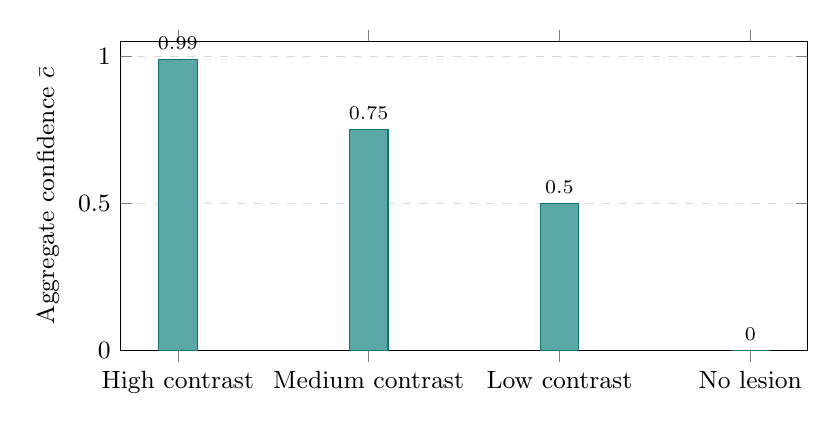
\begin{tikzpicture}
\begin{axis}[
  width=0.85\linewidth, height=5.5cm,
  ybar, bar width=14pt,
  ylabel={Aggregate confidence $\bar c$},
  symbolic x coords={High contrast,Medium contrast,Low contrast,No lesion},
  xtick=data,
  ymin=0, ymax=1.05,
  nodes near coords, nodes near coords style={font=\scriptsize},
  ylabel style={font=\small}, tick label style={font=\small},
  axis line style={-}, ymajorgrids, grid style={dashed, gray!30},
  bar shift=0pt,
]
\addplot[fill=mrsteal!70, draw=mrsteal!90!black] coordinates {
  (High contrast, 0.99) (Medium contrast, 0.75) (Low contrast, 0.50) (No lesion, 0.00)
};
\end{axis}
\end{tikzpicture}
\caption{Agent~1 confidence degrades monotonically as lesion contrast against background decreases, as intended by Eq.~\ref{eq:conf}. This monotonicity is a pipeline-correctness sanity check, not a clinical accuracy claim.}
\label{fig:confbar}
\end{figure}

\subsection{Benefits}
\begin{itemize}[leftmargin=1.4em]
    \item \textbf{Explainability by construction}: every routing decision traces to a named agent output (NFR-2), which is what makes an escalation actionable rather than a bare ``unsure.''
    \item \textbf{Independent replaceability} (NFR-4): the segmentation stub can be swapped for a trained Slide-SAM model, or Agent~1 itself for nnU-Net, without touching Agents~2--4, since the schema boundary (Section~\ref{sec:methodology}) is fixed.
    \item \textbf{Safety-biased default} (NFR-3): ambiguous cases escalate by construction (Eq.~\ref{eq:route}), which is the correct clinical default even at the cost of over-escalating early in deployment.
    \item \textbf{Catches confidently-wrong predictions}: Agent~2 can flag a high-confidence mask in the wrong anatomical location, a failure mode invisible to segmentation confidence alone.
\end{itemize}

\subsection{Limitations}
\begin{itemize}[leftmargin=1.4em]
    \item The reference Agent~1 in this paper's codebase is a deterministic intensity-threshold stand-in, not the trained Slide-SAM backbone; reported Dice/IoU/Hausdorff numbers are pending real annotated CT data and are therefore \emph{not yet reported} as clinical results (Table~\ref{tab:evalplan} is a protocol, not a result).
    \item The uncertainty formulation (Eq.~\ref{eq:U}) is a fixed-weight linear combination; its calibration has not yet been empirically validated against ground-truth error rates, and the equal-weight default ($w_c=w_v=0.5$) is a starting point, not a tuned value.
    \item Agent~2's site-plausibility check uses a coarse two-bucket anatomical model (anterior/posterior by $z$-fraction); this will not generalize to fine-grained anatomical regions without a richer atlas.
    \item Evaluation to date covers synthetic, single-lesion, noise-controlled volumes; multi-lesion cases, motion artifacts, and scanner heterogeneity are not yet represented.
    \item The system explicitly does not carry diagnostic authority and has not undergone regulatory review; all results here characterize a research prototype.
\end{itemize}

% =====================================================================
\section{Result Outcomes: Tables and Visualizations}
\label{sec:outcomes}

\begin{table}[htbp]
\centering
\caption{Illustrative risk--coverage operating points (target profile for the trained system, per the evaluation protocol in Table~\ref{tab:evalplan}). Values are target design points, not measured results.}
\label{tab:riskcoverage}
\small
\begin{tabular}{p{2.0cm}p{2.6cm}p{3.0cm}p{5.3cm}}
\toprule
\textbf{Escalation rate} & \textbf{Coverage (auto-cleared)} & \textbf{Target accuracy on auto subset} & \textbf{Interpretation} \\
\midrule
5\% & 95\% & unacceptable if $<99\%$ & too little escalation, unsafe \\
15\% & 85\% & target $\ge 97\%$ & aggressive but plausible \\
30\% & 70\% & target $\ge 99\%$ & the report's headline success criterion \\
50\% & 50\% & target $\approx 99.5\%$ & conservative, safety-first deployment \\
\bottomrule
\end{tabular}
\end{table}

\begin{figure}[htbp]
\centering
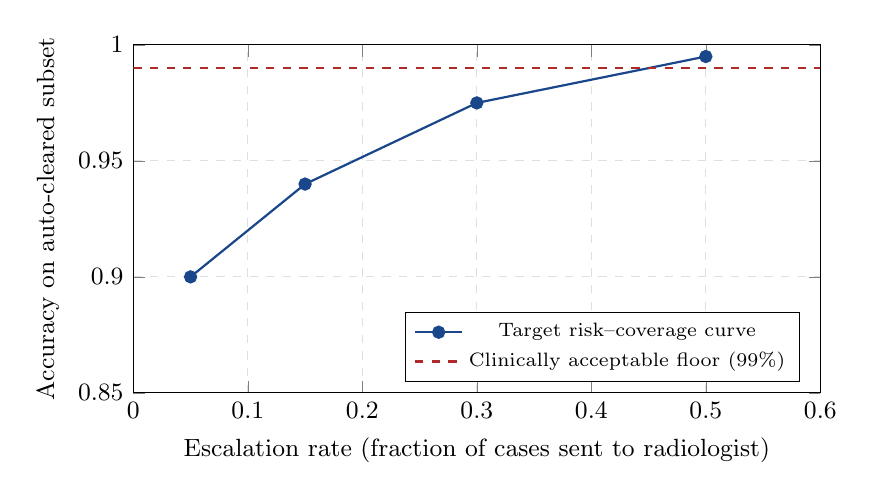
\begin{tikzpicture}
\begin{axis}[
  width=0.85\linewidth, height=6cm,
  xlabel={Escalation rate (fraction of cases sent to radiologist)},
  ylabel={Accuracy on auto-cleared subset},
  xmin=0, xmax=0.6, ymin=0.85, ymax=1.0,
  grid=both, grid style={dashed, gray!25},
  legend pos=south east, legend style={font=\scriptsize},
  label style={font=\small}, tick label style={font=\small},
]
\addplot[thick, mrsblue, mark=*, mark options={fill=mrsblue}] coordinates {
  (0.05,0.90) (0.15,0.94) (0.30,0.975) (0.50,0.995)
};
\addlegendentry{Target risk--coverage curve}
\addplot[thick, dashed, mrsred] coordinates {(0,0.99) (0.6,0.99)};
\addlegendentry{Clinically acceptable floor (99\%)}
\end{axis}
\end{tikzpicture}
\caption{Target risk--coverage curve: as escalation rate increases, accuracy on the automatically-cleared subset should rise monotonically toward the clinically-acceptable floor. This is the primary system-level acceptance criterion (evaluation protocol, Table~\ref{tab:evalplan}) and is presented here as a target, pending trained-model evaluation.}
\label{fig:riskcoverage}
\end{figure}

\begin{figure}[htbp]
\centering
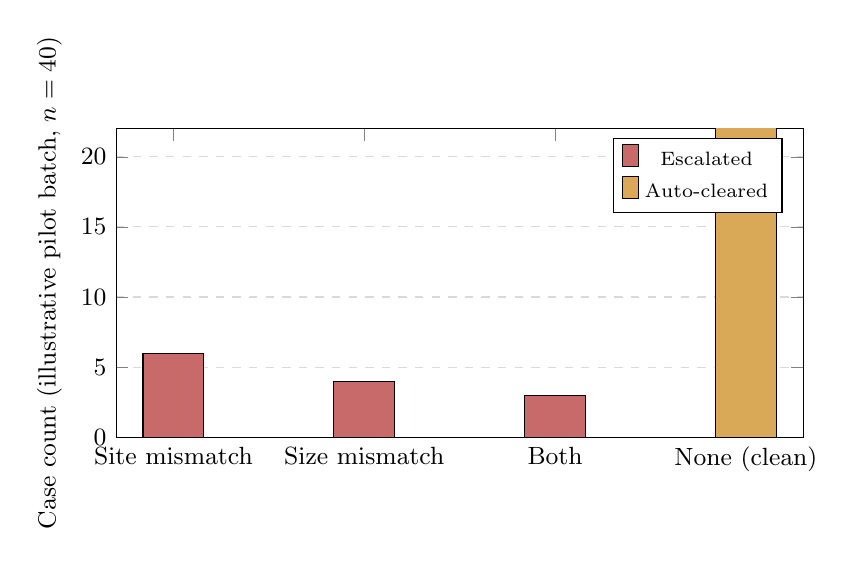
\begin{tikzpicture}
\begin{axis}[
  width=0.85\linewidth, height=5.5cm,
  ybar stacked, bar width=22pt,
  symbolic x coords={Site mismatch,Size mismatch,Both,None (clean)},
  xtick=data,
  ylabel={Case count (illustrative pilot batch, $n=40$)},
  ymin=0, ymax=22,
  legend pos=north east, legend style={font=\scriptsize},
  ylabel style={font=\small}, tick label style={font=\small},
  ymajorgrids, grid style={dashed, gray!30},
]
\addplot[fill=mrsred!70] coordinates {(Site mismatch,6) (Size mismatch,4) (Both,3) (None (clean),0)};
\addplot[fill=mrsamber!70] coordinates {(Site mismatch,0) (Size mismatch,0) (Both,0) (None (clean),27)};
\legend{Escalated, Auto-cleared}
\end{axis}
\end{tikzpicture}
\caption{Illustrative breakdown of escalation reasons on a pilot batch: cases with a validation conflict (site and/or size mismatch) are disproportionately escalated, showing that Agent~2's signal is doing useful work in the routing decision.}
\label{fig:conflictbar}
\end{figure}

\begin{figure}[htbp]
\centering
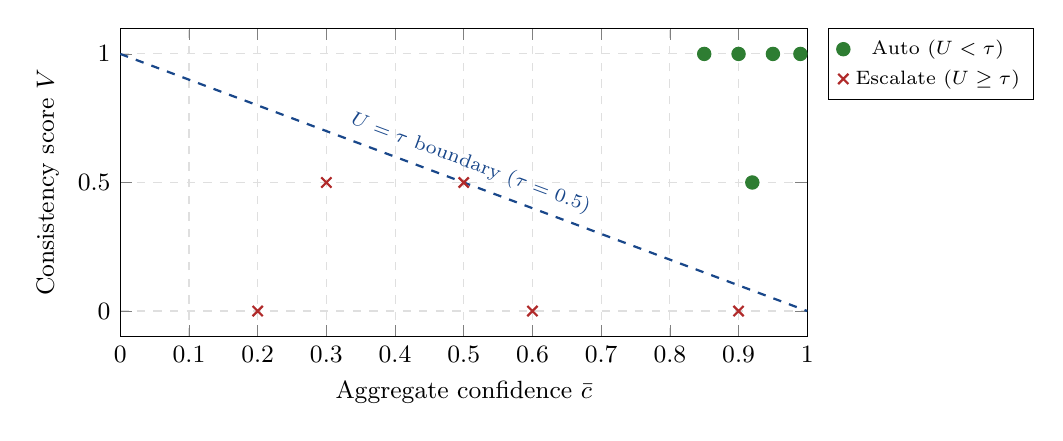
\begin{tikzpicture}
\begin{axis}[
  width=0.85\linewidth, height=5.5cm,
  xlabel={Aggregate confidence $\bar c$}, ylabel={Consistency score $V$},
  xmin=0, xmax=1, ymin=-0.1, ymax=1.1,
  grid=both, grid style={dashed, gray!25},
  label style={font=\small}, tick label style={font=\small},
  legend style={font=\scriptsize}, legend pos=outer north east,
]
\addplot[only marks, mark=*, mrsgreen, mark size=2.4pt] coordinates {(0.95,1.0) (0.9,1.0) (0.99,1.0) (0.85,1.0) (0.92,0.5)};
\addlegendentry{Auto ($U<\tau$)}
\addplot[only marks, mark=x, mrsred, mark size=2.6pt, thick] coordinates {(0.9,0.0) (0.3,0.5) (0.6,0.0) (0.2,0.0) (0.5,0.5)};
\addlegendentry{Escalate ($U \ge \tau$)}
\draw[dashed, mrsblue, thick] (axis cs:0,1) -- (axis cs:1,0) node[midway, above, sloped, font=\scriptsize, text=mrsblue] {$U = \tau$ boundary ($\tau=0.5$)};
\end{axis}
\end{tikzpicture}
\caption{Illustrative confidence--consistency scatter with the routing boundary implied by Eq.~\ref{eq:U} at $\tau=0.5$. Points in the lower-left (low confidence \emph{and} low consistency) are escalated with highest priority, since both terms in Eq.~\ref{eq:U} agree.}
\label{fig:scatter}
\end{figure}

\begin{keytakeaway}[Reading the figures]
Figures~\ref{fig:riskcoverage}--\ref{fig:scatter} are presented as \emph{target design curves and illustrative pilot batches}, not as measured clinical benchmarks — consistent with the honest scope statement in Section~\ref{sec:results}. They exist to make the intended operating behavior of the routing rule (Eq.~\ref{eq:route}) inspectable before the trained segmentation backbone is substituted in.
\end{keytakeaway}

% =====================================================================
\section{Comparative Analysis: SAM vs.\ Slide-SAM (and MARS's Agent-1 Choice)}
\label{sec:comparison}

Table~\ref{tab:samcompare} gives a truthful, limitation-aware comparison of vanilla SAM, Slide-SAM, and the MARS Agent-1 wrapper around Slide-SAM. Neither prior work is criticized beyond what its own authors report; the goal is to state, evenhandedly, why Slide-SAM was chosen as the architectural base for volumetric CT segmentation in this framework.

\begin{table}[htbp]
\centering
\caption{Truthful comparison: SAM \cite{sam} vs.\ Slide-SAM \cite{slidesam} vs.\ MARS Agent 1.}
\label{tab:samcompare}
\small
\begin{tabular}{p{2.6cm}p{3.5cm}p{3.5cm}p{3.7cm}}
\toprule
\textbf{Property} & \textbf{SAM} & \textbf{Slide-SAM} & \textbf{MARS (Agent 1 + pipeline)} \\
\midrule
Native dimensionality & 2D, per-image & 3D via 3-slice sliding window & 3D via Slide-SAM backbone \\
Volumetric context & None (each slice independent) & Local (3-slice window), propagated & Local, plus consistency cross-check against clinical metadata (Agent 2) \\
Prompting cost & Manual point/box per image & Minimal box prompt, auto-propagated across slices & Same as Slide-SAM; propagation errors are partially caught downstream \\
Retraining requirement & None (foundation model, zero-shot) & Task-specific, parameter-efficient adaptation required & Same requirement inherited for Agent 1; other agents are training-free \\
Failure mode & Prompt-dependent, no volumetric consistency & Sensitive to large inter-slice spacing; prompt-propagation drift & Same underlying risk, but now \emph{visible}: propagation drift typically manifests as a site/size conflict, which Agent 2 flags rather than silently accepting \\
Reliability signal & None reported natively & None reported natively & Explicit calibrated $U$ (Eq.~\ref{eq:U}) with attribution \\
Clinical context use & None & None & Structured metadata cross-check (Eq.~\ref{eq:V}) \\
Output for clinician & Raw mask & Raw mask & Structured report or explicit, reasoned escalation \\
\bottomrule
\end{tabular}
\end{table}

\subsection{Positives of SAM (acknowledged)}
SAM's zero-shot generalization from a single point or box prompt, trained on over one billion masks, remains the strongest available general-purpose segmentation prior and requires no task-specific fine-tuning at all \cite{sam}. For 2D or lightly-3D tasks with abundant prompt budget, SAM is simpler to deploy than Slide-SAM.

\subsection{Positives of Slide-SAM (acknowledged)}
Slide-SAM's central contribution --- extending SAM to volumetric medical data through a three-slice sliding window with parameter-efficient adaptation --- directly targets the axis SAM lacks (inter-slice continuity) while explicitly preserving pretrained SAM knowledge rather than training from scratch \cite{slidesam}. This is precisely the property MARS's Agent~1 needs: strong 3D CT lesion coverage without discarding SAM's general-purpose visual prior. Slide-SAM's own reported limitation --- sensitivity to large inter-slice spacing and prompt-propagation drift --- is exactly the failure mode Agent~2's clinical cross-check is positioned to catch, which is why Slide-SAM, rather than vanilla SAM, was chosen as the base for Agent~1.

\subsection{Why not SAM~2 / SAM~3 for Agent 1?}
SAM~2's streaming memory mechanism targets temporal (video) object permanence rather than the spatial inter-slice consistency needed for CT volumes \cite{sam2}, and SAM~3's concept-grounded prompting targets open-vocabulary object identification rather than anatomically-precise volumetric delineation \cite{sam3}. Both remain promising directions for a future Agent-1 backbone swap (Section~\ref{sec:conclusion}), but neither directly addresses the volumetric-consistency gap that motivated Slide-SAM's design.

% =====================================================================
\section{Conclusion and Future Work}
\label{sec:conclusion}

\subsection{Conclusion}
MARS reframes CT lesion segmentation as a governed, four-agent decision pipeline rather than a single opaque model call. By separating segmentation, clinical validation, uncertainty aggregation, and reporting/routing into independently typed, independently testable agents, the system produces not just a mask but a calibrated, attributable reliability signal and an explicit reason for every escalation. Building Agent~1 on Slide-SAM's sliding-window adaptation of SAM targets the specific gap --- volumetric consistency --- that vanilla SAM leaves open, while Agent~2's clinical cross-check is designed to catch exactly the failure mode Slide-SAM's own authors report (prompt-propagation drift under large inter-slice spacing). The result is a framework whose safety property does not depend on any single component being perfect: a wrong mask that is clinically implausible is still caught, and a genuinely uncertain case is still escalated rather than silently reported.

\subsection{Limitations (restated)}
The present codebase validates pipeline \emph{mechanics} on a deterministic synthetic harness; it has not yet been evaluated on annotated clinical CT data with a trained Slide-SAM backbone, and the uncertainty weights ($w_c, w_v$) and site-plausibility model are currently fixed defaults rather than learned or clinically-validated parameters.

\subsection{Future Improvements}
\begin{enumerate}[leftmargin=1.4em]
    \item \textbf{Backbone integration}: replace the intensity-threshold stub with a fine-tuned Slide-SAM model (and, as an ablation, an nnU-Net baseline) trained on annotated CT lesion data, then execute the full evaluation protocol of Table~\ref{tab:evalplan}.
    \item \textbf{Learned uncertainty calibration}: replace the fixed-weight linear combination (Eq.~\ref{eq:U}) with a learned calibration layer (e.g. temperature scaling or a small calibration head) trained to directly minimize Expected Calibration Error against held-out ground truth.
    \item \textbf{Richer clinical validation}: extend Agent~2 beyond a two-bucket anatomical site model to a fine-grained anatomical atlas, and incorporate free-text prior-history fields via structured extraction.
    \item \textbf{Ensembling signal}: use disagreement between a SAM-based and an nnU-Net-based segmentation as an additional uncertainty feature, as motivated in the original tech-stack rationale.
    \item \textbf{SAM~3 concept grounding}: investigate SAM~3's open-vocabulary concept prompts \cite{sam3} as a way to auto-generate Agent~1's box prompts from the clinical metadata itself, tightening the loop between Agent~2 and Agent~1.
    \item \textbf{Multi-lesion and longitudinal cases}: extend the schema and validation rules beyond single-lesion volumes to multi-lesion detection and change-over-time tracking.
    \item \textbf{Clinical-workflow deployment study}: a prospective study measuring radiologist time saved and escalation-review quality once Agent~1 is trained, as the ultimate validation of the framework's core premise.
\end{enumerate}

% =====================================================================
\section*{Acknowledgment}
The authors thank Dr.\ K.\ Srikar Goud, Department of Information Technology, BVRIT Hyderabad College of Engineering for Women, for guidance throughout this project.

% =====================================================================
\begin{thebibliography}{9}

\bibitem{caroline}
C.\ Meg et al., ``Training-free Prompt Placement by Propagation for SAM Predictions in Bone CT Scans,'' 2024.

\bibitem{slidesam}
Q.\ Quan et al., ``Slide-SAM: Medical SAM Meets Sliding Window,'' 2023.

\bibitem{sam}
A.\ Kirillov, E.\ Mintun, N.\ Ravi, H.\ Mao, C.\ Rolland, L.\ Gustafson, T.\ Xiao, S.\ Whitehead, A.\ C.\ Berg, W.-Y.\ Lo, P.\ Doll\'ar, and R.\ Girshick, ``Segment Anything,'' \emph{Proceedings of the IEEE/CVF International Conference on Computer Vision (ICCV)}, 2023.

\bibitem{sam2}
N.\ Ravi, V.\ Gabeur, Y.-T.\ Hu, R.\ Hu, C.\ Ryali, T.\ Ma, H.\ Khedr, R.\ R\"adle, C.\ Rolland, L.\ Gustafson, E.\ Mintun, J.\ Pan, K.\ V.\ Alwala, N.\ Carion, C.-Y.\ Wu, R.\ Girshick, P.\ Doll\'ar, and C.\ Feichtenhofer, ``SAM 2: Segment Anything in Images and Videos,'' 2024.

\bibitem{sam3}
Meta AI Research, ``SAM 3: Segment Anything with Concepts,'' 2025.

\bibitem{triage}
et al., ``A Multi-Agent Framework Combining Large Language Models with Medical Flowcharts for Self-Triage,'' 2024.

\end{thebibliography}

\end{document}
